\documentclass[12pt]{article}

\title{CSpace: Interactive Exploration of Chemical Spaces}
\author{Ryan Jenkins}
\usepackage[a4paper, left=1.5in, right=1in, top=1in, bottom=1in]{geometry}
\usepackage[document]{ragged2e}
\usepackage{cite}
\usepackage{subfig}
\usepackage{float}
\usepackage{graphicx}
\graphicspath{ {img/} }
\usepackage[font={small,it}]{caption}
\usepackage [english]{babel}
\usepackage [autostyle, english = american]{csquotes}
\MakeOuterQuote{"}
\linespread{1.5}
\setlength{\parindent}{0in}
\setlength{\parskip}{16pt plus4pt minus 4pt}

\begin{document}

\maketitle

\begin{abstract}
Analysis of similarity of novel chemicals to chemicals with known physiological effects and known mechanisms of action plays an important role in drug discovery, and studying relationships between known chemicals can yield significant insights into the relationship between chemical structure and interaction. CSpace is an interactive tool for visualizing and exploring "chemical spaces", embeddings of sets of chemicals into low dimensional spaces under some similarity metric.
\end{abstract}

\newpage
\section{Introduction}
While it is widely understood that similarity of chemical structure does not always equate to similarity of effect or interaction, the notion of chemical similarity has nevertheless been successfully studied and employed in domains like drug discovery\cite{Nikolova2003}. The notion of chemical similarity or chemical "distance" naturally gives rise to a notion of chemical "space", an abstract space wherein points represent possible chemical structures or some facet of chemical structure.

CSpace is a tool for interactively visualizing chemical spaces in three dimensions with the goal of providing insight into the organization of large groups of chemicals and the relationship between chemical structure and effect.

\section{CSpace Concepts/Structure}
The most basic record in CSpace is a chemical. Chemical structure is stored internally as a Simplified Molecular Input Line Entry System(SMILES) string\cite{Weininger1988}. Chemicals records also contain various optional metadata including the IUPAC name and PubChem CID. Each chemical may have one or more tags which have no semantic meaning within the system but are used during presentation, e.g. caffeine can be tagged as a purine and as a CNS stimulant.

CSpace currently supports importing chemicals from structure-data files(SDF) which wrap a collection of data in the MDL molfile format. PubChem offers a wealth of chemical information retrievable in the SDF format.

Chemicals are aggregated into "chemical sets", typically by taking the union of chemicals holding any of a some set of tags, e.g. a chemical set of the nitrogenous bases may be formed from the from purine and pyrimidine tags.

A chemical set may have multiple "facets". A facet is an embedding of the chemicals in a set to a 3 dimensional euclidean space. The identify of a facet is formed by its chemical set, a similarity metric for use between chemicals, and an embedding strategy. Chemical set facets are the central object which CSpace visualizes.

\section{Algorithms Used}
Creating chemical set facets is a central task for CSpace. The supported similarity metrics and embedding algorithms on a chemical set are briefly described below.

\subsection{Similarity Metrics}
Currently two similarity metrics are supported: RDKit and Gobbi-Poppinger substructure fingerprints.

The RDKit fingerprinting algorithm\cite{landrum_2007} is a modified formulation of the Daylight chemical fingerprinting algorithm\cite{daylighttheorymanual_2019}. Like the Daylight algorithm, it operates by enumerating and counting paths through the atom/bond graph of a molecule, by default considering all paths between 1 and 7 bonds in length. The identity of a bond path (for the purposes of counting) consists of the atomic weight of the atoms participating in each bond and the aromaticity of the bond. These bond path histograms are then hashed to produce a fixed length bit vector that summarizes the structure of the chemical.

The Gobbi-Poppinger fingerprinting algorithm\cite{Gobbi1998} operates on a similar premise to the RDKit algorithm, however rather than enumerating and counting all possible bond paths within some range of sizes, it is instead equipped with a fixed library of substructure patterns which are identified and counted in molecules. This produces a smaller histogram of substructures, however the structures are selected to be chemically meaningful pharmacophores. These histograms are hashed in a similar manner to the RDKit approach and also yield a fixed length bit vector.

After chemicals fingerprints are computed, a distance matrix $D$ is computed:

\begin{equation}
  D_{i,j} = 1 - T(i,j)
\end{equation}

Where $T(i,j)$ is the Tanimoto coefficient between molecules $i$ and $j$ in the chemical set.

\subsection{Embedding Approaches}
CSpace currently supports a total of 5 embedding techniques. They are: metric and non-metric variants of Classical Multi-Dimensional Scaling and SMACOF, as well as t-distributed Stochastic Neighbor Embedding(t-SNE).

The goal of all five methods is to create an n-dimensional (3, in our case) set of points from a dissimilarity matrix where inter-point distances are in some sense preserved. Metric MDS and SMACOF both achieve this by minimizing the difference in inter-point distances (strain) in the embedding with respect to the original distance matrix. The non-metric variants of these two techniques attempt to maintain the relative ordering for pair-wise distance rather than globally minimizing stress (e.g. if $D_{i,j} < D_{i,k}$ than for embedded point $E_i$ it holds that $||E_i - E_j|| < ||E_i - E_k||$ for all $i, j, k$).

t-SNE is a non-linear embedding technique that balances minimization of strain in near-by clusters of points and inter-cluster distances\cite{maaten2008visualizing}.

\section{Examples}
As there is not singularly correct notion of chemical similarity, accordingly there is no singular objective measure of the correctness of a CSpace embedding. One useful property of an embedding would be that similarity of effect in humans between two chemicals corresponds proximity in an embedded space, although other criteria for proximity may be useful (e.g. proximate chemicals have a similar method of synthesis, or similar level of toxicity regardless of other effects). In this section we will look at examples of embeddings generated by CSpace and make the case for their general plausibility. To this end we will look at two chemical sets collected from PubChem.

\subsection{Classes of Chemicals Containing Frequent Recreational Drugs}
This dataset of 1030 compounds consists of 469 benzodiazepines, 251 amphetamines, 136 opiates, and 184 ergolines. Note that these four classes were selected because they contain chemicals frequently used recreationally, however membership in the class is defined chemically. For example 3-[5-(3-Nitro-phenyl)-furan-2-yl]-2-(piperidine-1-carbonyl)-acrylonitrile is categorized as an opiate under the Anatomical Therapeutic Chemical Classification System but is not commonly synthesized or used recreationally.

\begin{figure}[H]
  \centering
  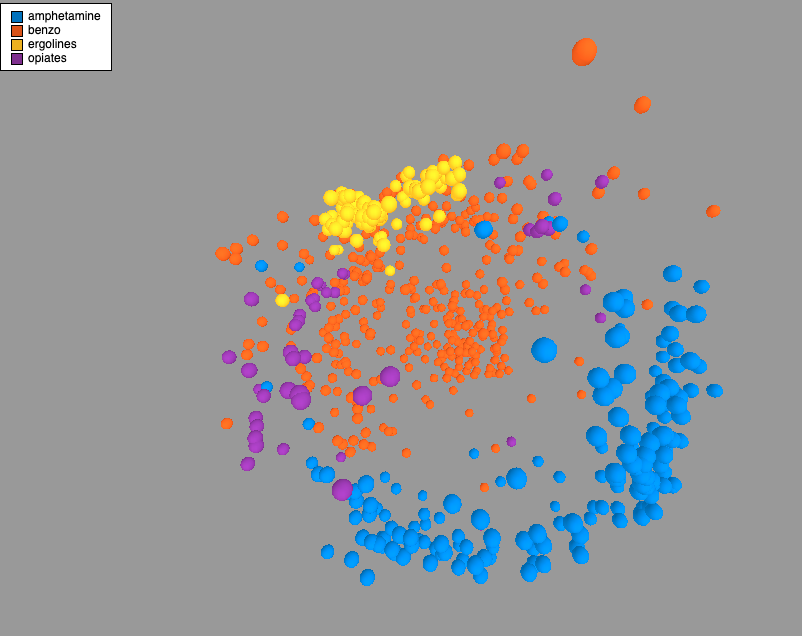
\includegraphics[width=\textwidth]{rec-rdk-mds}
  \captionsetup{justification=centering}
  \caption{Recreational classes under RDK fingerprinting and metric MDS}
\end{figure}

Figure 1 shows the MDS embedding of Tanimoto/RDKit fingerprints for this dataset.  Here we see good separation between the amphetamines, benzodiazepines,  and ergolines. The opiates group is a little more spread out but generally closer to the benzodiazepine group. Interestingly the ergoline group, which contains stimulants, is also positioned closer to both benzodiazepines and opiates than amphetamines. A likely explanation for this is that these three classes of compounds are all more complex and generally heavier than amphetamines.

\begin{figure}[H]
  \centering
  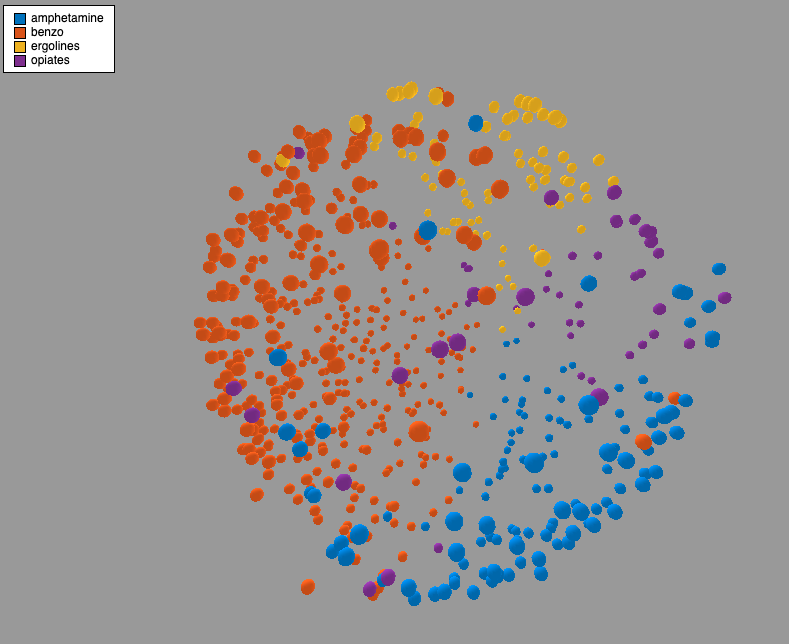
\includegraphics[width=\textwidth]{rec-gobbi-mds}
  \captionsetup{justification=centering}
  \caption{Recreational classes under Gobbi-Poppinger and metric MDS}
\end{figure}

The Gobbi-Poppinger/Tanimoto similarity measure produces similar results to RDK fingerprinting although it differentiates members of each class over more space while maintaining fairly clean separation, as seen in figure 2.

\begin{figure}[H]
  \begin{tabular}{cc}
    \subfloat[TSNE]{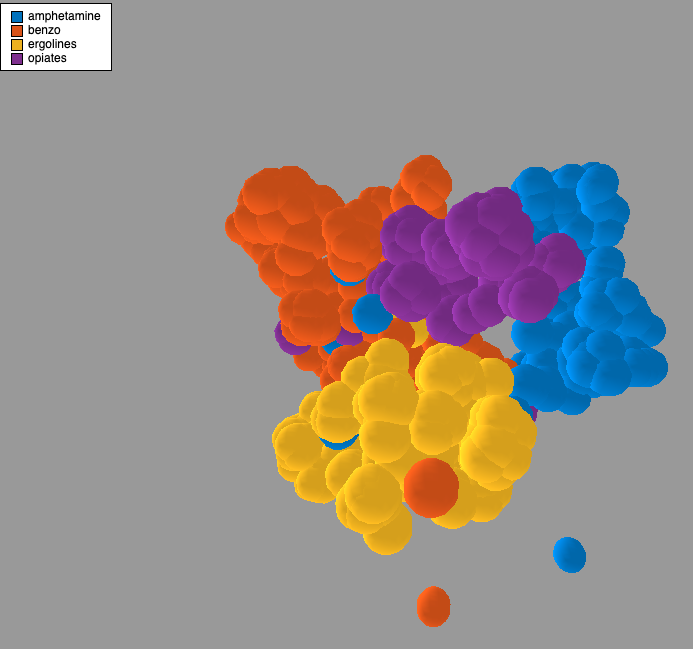
\includegraphics[height = 2in]{rec-rdk-tsne}} &
    \subfloat[SMACOF]{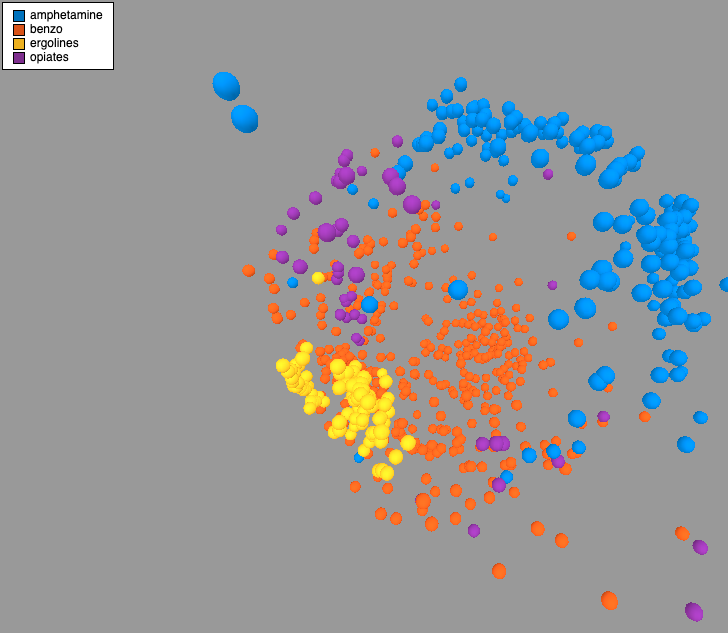
\includegraphics[height = 2in]{rec-rdk-smacof}}\\
    \subfloat[Non-metric MDS]{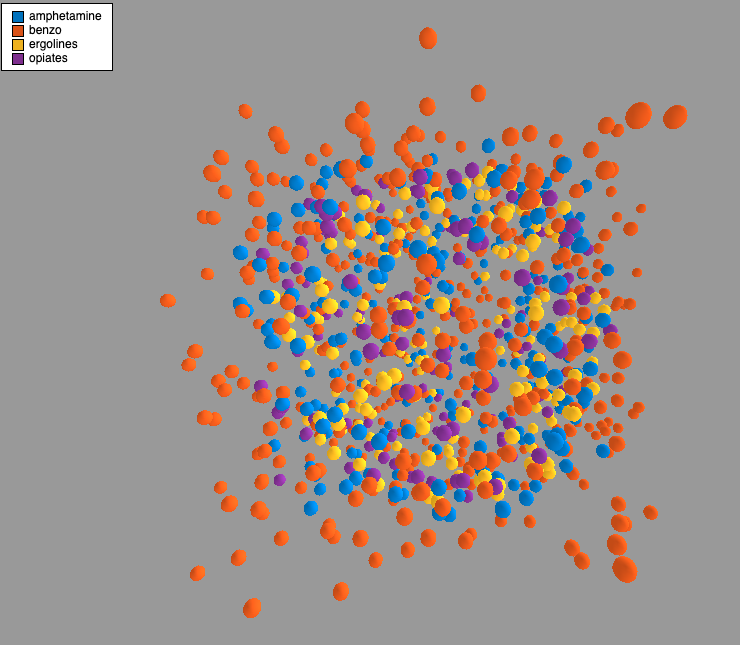
\includegraphics[height = 2in]{rec-rdk-nmmds}} &
    \subfloat[Non-metric SMACOF]{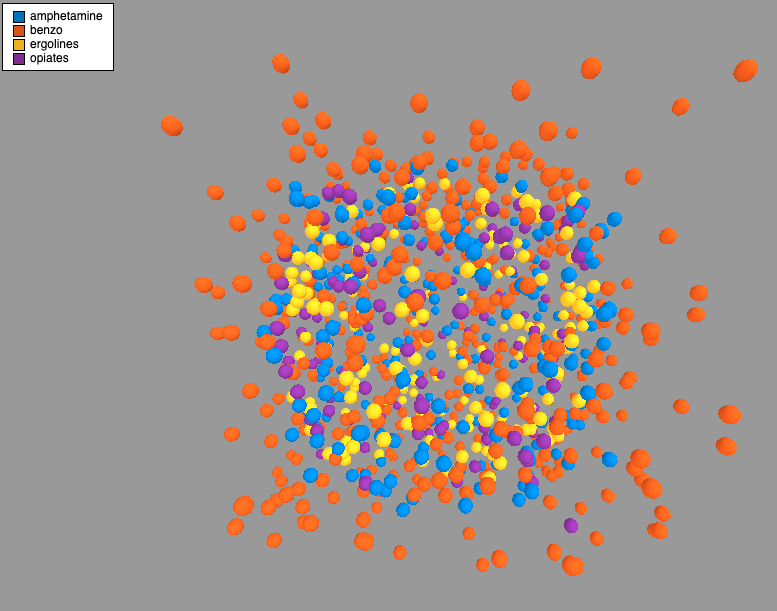
\includegraphics[height = 2in]{rec-rdk-nmsmacof}}
  \end{tabular}
  \captionsetup{justification=centering}
  \caption{Four embedding strategies for the recreational dataset}
\end{figure}

Figure 3 shows the four remaining embedding techniques all with the RDKit fingerprinting similarity metric. TSNE produces tighter cluster of chemicals with a few more wide outliers than MDS. Notably it groups the opiates class into a much tighter cluster than MDS. I speculate that this is because opiates are the smallest class in the dataset, global embeddings like MDS can minimize global stress while still distorting the distance relationships between members of a small class, whereas TSNE prioritizes maintaining local distance relationships.

Note that the SMACOF plot looks nearly identical to the MDS plot, and that non-metric variants of both SMACOF and MDS are nearly the same. This is a trend that holds across datasets, and as such only MDS will be considered in following sections. Also notice that non-metric variants show almost no class separation, the reason for this is not understood at this point.

\subsection{Clinical Sedatives and Psychostimulants}
This set of 289 compounds consists of 120 chemicals identified as psychostimulants and 169 sedatives, corresponding to the N06B and N05C categories of the Anatomical Therapeutic Chemical Classification System. Unlike the previous dataset, these classes are only defined by their therapeutic uses and are therefore more structurally diverse.

\begin{figure}[H]
  \centering
  \begin{tabular}{cc}
    \subfloat[RDKit/MDS]{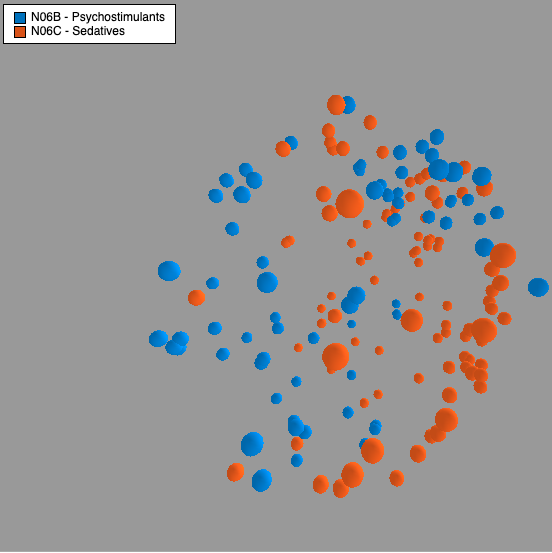
\includegraphics[height = 2in]{sp-rdk-mds}} &
    \subfloat[RDKit/TSNE]{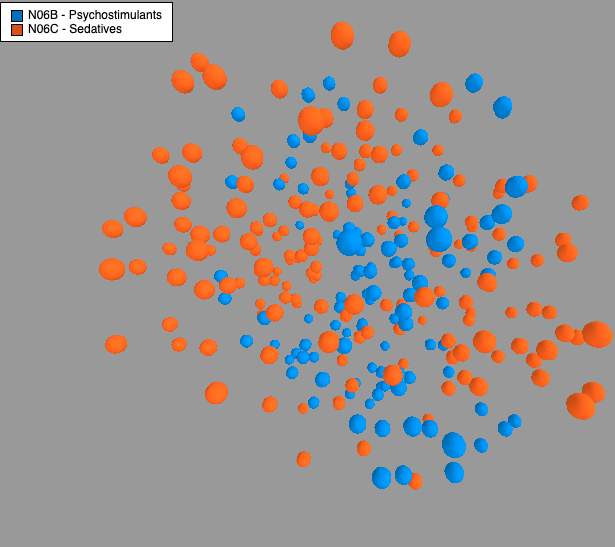
\includegraphics[height = 2in]{sp-rdk-tsne}}\\
    \subfloat[Gobbi/MDS]{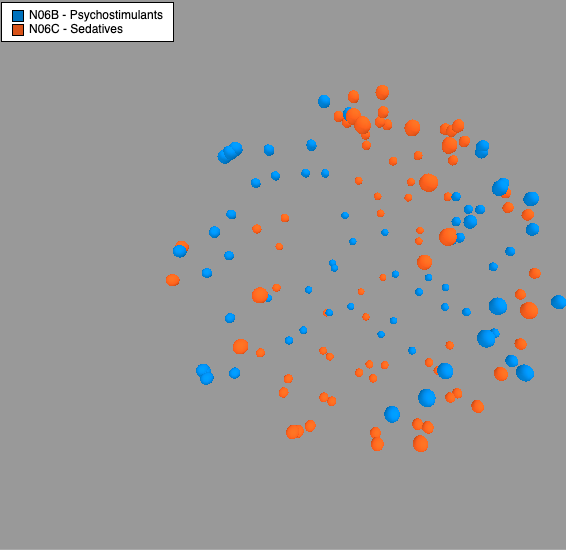
\includegraphics[height = 2in]{sp-gobbi-mds}} &
    \subfloat[Gobbi/TSNE]{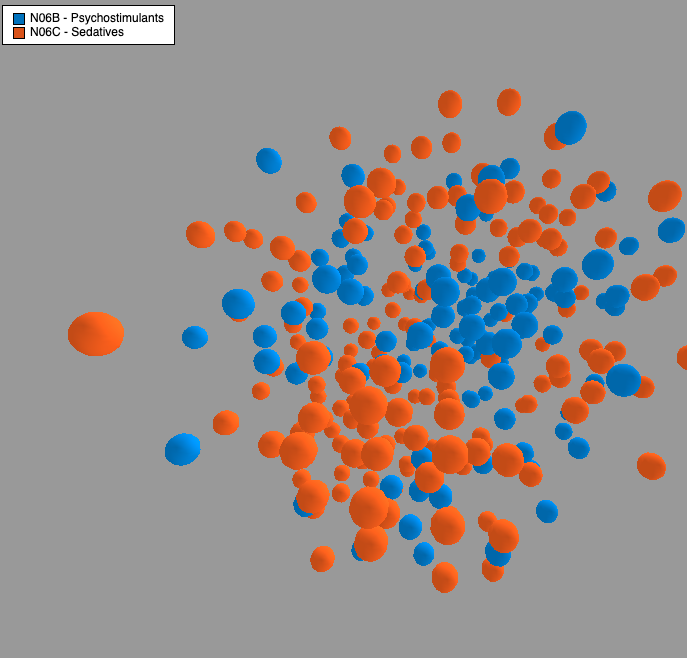
\includegraphics[height = 2in]{sp-gobbi-tsne}}
  \end{tabular}
  \captionsetup{justification=centering}
  \caption{Three embeddings of the sedatives and psychostimulants chemical set}
\end{figure}

As we can see from figure 4, this dataset yields only weak separation between classes for all similarity metrics and embeddings. TSNE remains prone to producing outlying points. This is reasonable given the character of data as being categorized by therapeutic use rather than chemical structure.

\section{Conclusion}
The CSpace application allows for visualization of chemical spaces. The algorithms currently employed seem to model structural similarity well and can produce interesting visualizations however this does not translate to \textit{in vivo} effect particularly well.

\newpage
\bibliography{cites}
\bibliographystyle{ieeetr}

\end{document}
